\subsection{Two Pool Experiment}

\begin{figure}[t!]
    \centering
	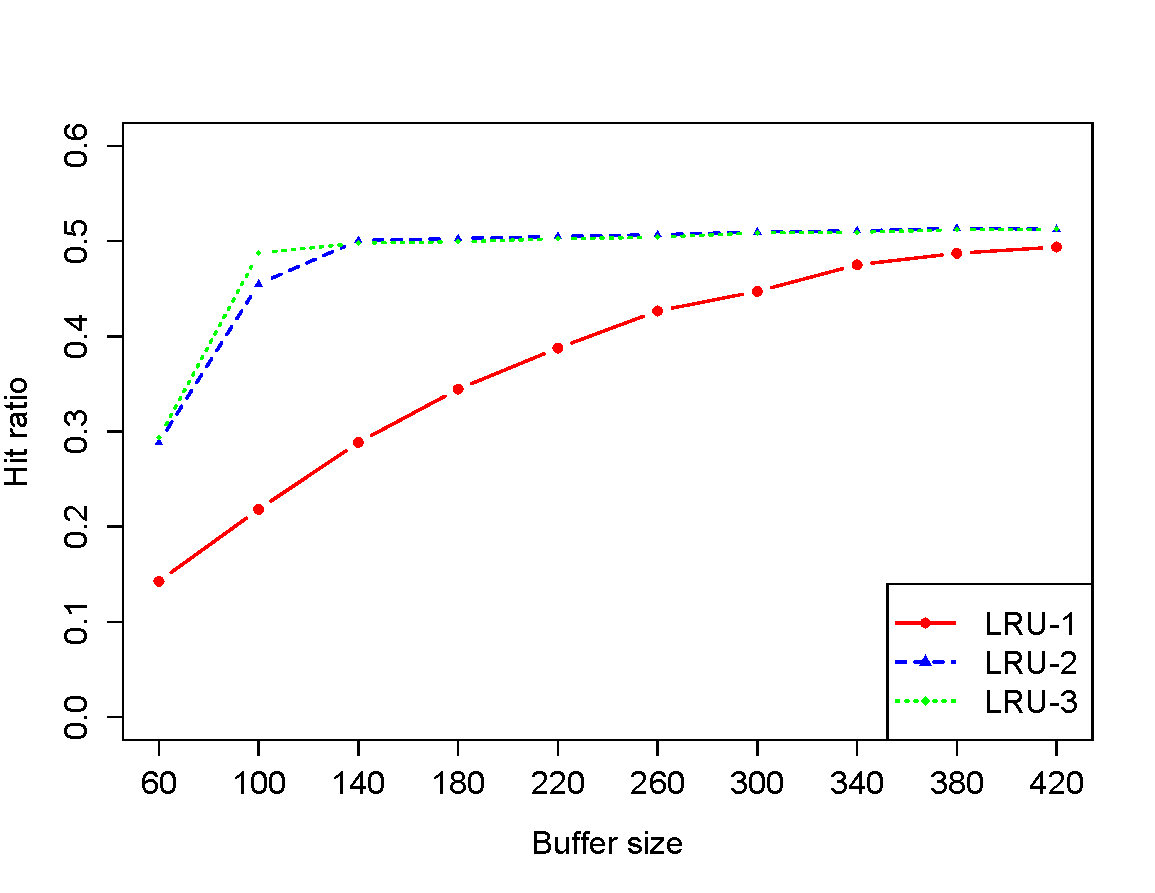
\includegraphics[width=0.5\textwidth]{./figures/two_pool.pdf}
	\caption{Simulation results of two pool experiment with disk page pools of $N_1 = 100$ pages and $N_2 = 10000$ pages. Horizontal axis shows the simulate buffer size and vertical axis shows measured hit ratio. All measurements were evaluated with Correlated Reference Period set to 0.}
	\label{fig:two_pool}
\end{figure}


\subsection{Zipfian Random Access Experiment}

\begin{figure}[t!]
    \centering
	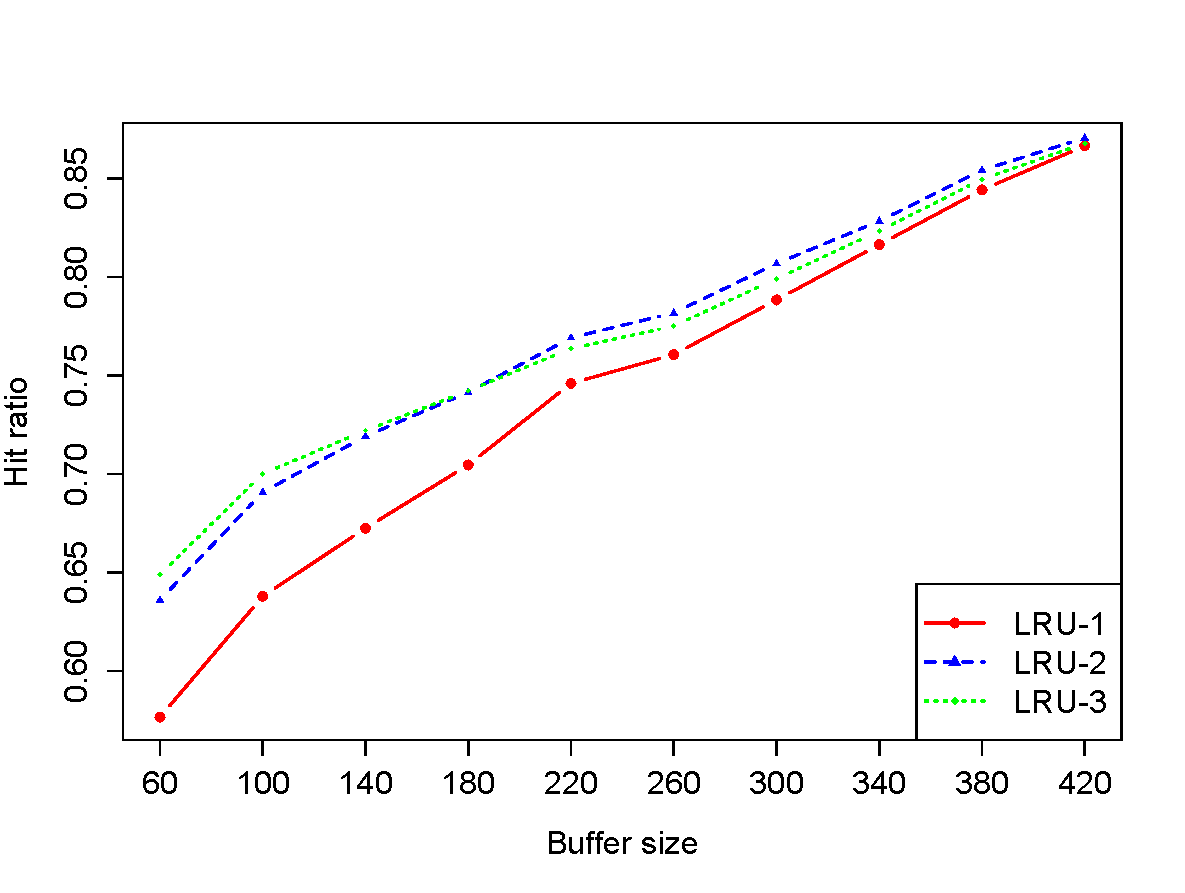
\includegraphics[width=0.5\textwidth]{./figures/zipfian.pdf}
	\caption{Simulation results of cache hit ratio for random access with Zipfian 80-20 distribution to $N = 1000$ pages in the pool. Horizontal axis shows the simulate buffer size and vertical axis shows measured hit ratio. All measurements were evaluated with Correlated Reference Period set to 0.}
	\label{fig:zipfian}
\end{figure}


\subsection{PostgreSQL Trace Experiment}

\begin{figure}[t!]
    \centering
	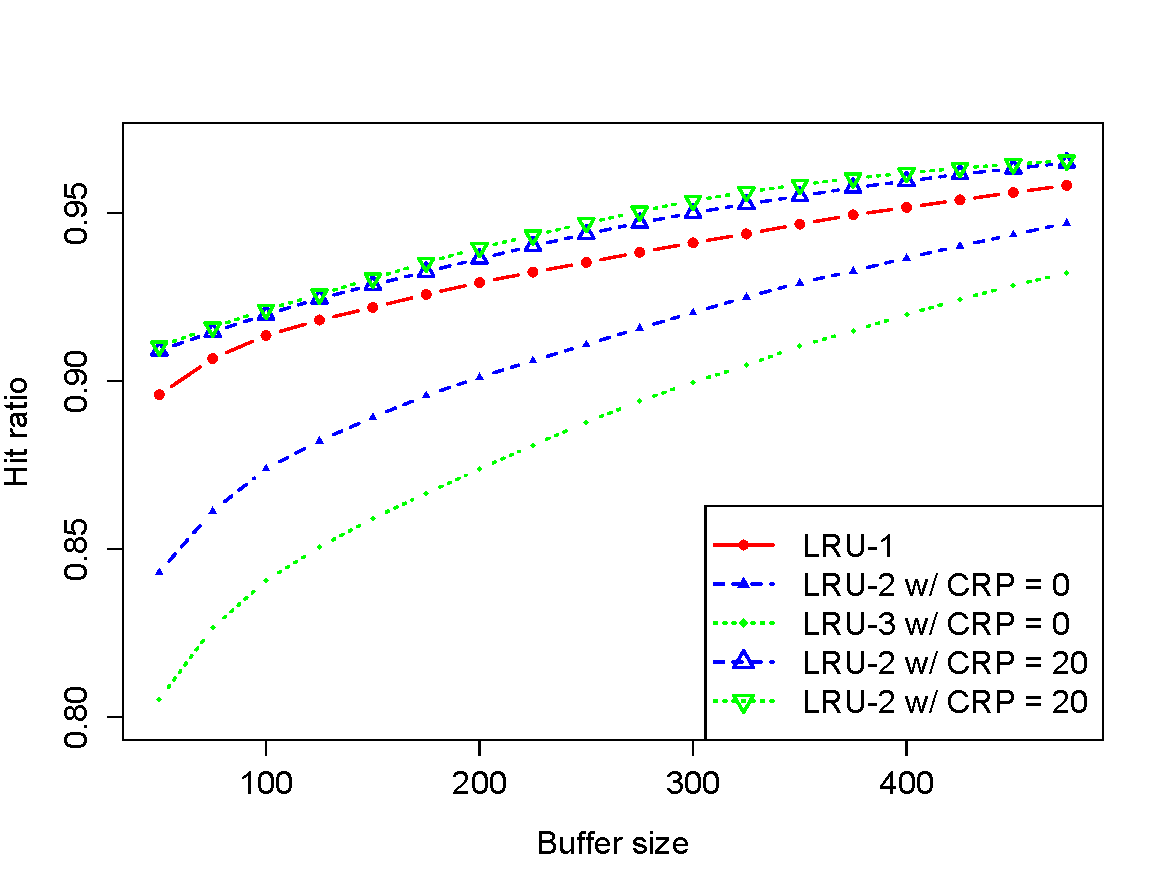
\includegraphics[width=0.5\textwidth]{./figures/postgres.pdf}
	\caption{Simulation results of different buffer management strategies using a trace collected from PostgreSQL running \texttt{pgbench} benchmark. Horizontal axis shows the simulate buffer size and vertical axis shows measured hit ratio. LRU-2 and LRU-3 are evaluated with Correlated Reference Period set to 0 and 20.}
\end{figure}
